%% LyX 2.1.0 created this file.  For more info, see http://www.lyx.org/.
%% Do not edit unless you really know what you are doing.
\documentclass[english]{beamer}
\usepackage[T1]{fontenc}
\usepackage[latin9]{inputenc}
\setcounter{secnumdepth}{3}
\setcounter{tocdepth}{3}
\usepackage{float}
\usepackage{graphicx}

\makeatletter
%%%%%%%%%%%%%%%%%%%%%%%%%%%%%% Textclass specific LaTeX commands.
 % this default might be overridden by plain title style
 \newcommand\makebeamertitle{\frame{\maketitle}}%
 % (ERT) argument for the TOC
 \AtBeginDocument{%
   \let\origtableofcontents=\tableofcontents
   \def\tableofcontents{\@ifnextchar[{\origtableofcontents}{\gobbletableofcontents}}
   \def\gobbletableofcontents#1{\origtableofcontents}
 }

\makeatother

\usepackage{babel}
\begin{document}
\begin{frame}{Modeling process}

\begin{itemize}
\item Number of words (V), number of topics (K)
\end{itemize}

\begin{figure}[H]
\begin{centering}
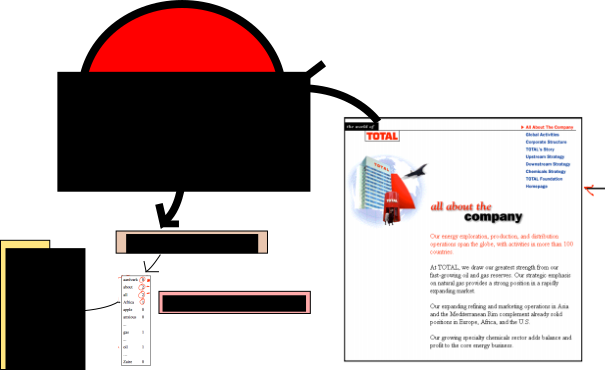
\includegraphics[scale=0.5]{piclol}\protect\caption{Admixture model}

\par\end{centering}

\end{figure}


\end{frame}

\begin{frame}{Task}


\begin{center}
{\huge{}The learning task is to find the word-topic matrix A with
the statistical model above. This is the essence of statistical recovery.
They also show how to learn the hyperparameters of the topic distribution
when it is a Dirichlet distribution}
\par\end{center}{\huge \par}

\end{frame}



\begin{frame}{Word-topic matrix}


\framesubtitle{Kristy's slide goes here}

\end{frame}

\begin{frame}{Topic recovery using Bayes' Rule}


\framesubtitle{Mathematical prerequisites}
\begin{itemize}
\item For any two words $w_{1}$and $w_{2}$ with respective topic assignments
$z_{1}$ and $z_{2}$ the elements of the word-topic matrix can be
interpreted as
\end{itemize}

$A_{i,k}=p(w_{1}=i\,|z_{1}=k)$$ $ (1)


The A matrix gives probability of word in the ith row given a topic
k (column)
\begin{itemize}
\item Word co-occurences

\begin{itemize}
\item Q $\rightarrow$ measures joint probability of words occuring together
\item $Q_{i,j}=p(w_{1}=i,w_{2}=j)$ (2)
\item $\bar{Q}_{i,j}=p(w_{2}=j|w_{1}=i$) (3)
\end{itemize}
\end{itemize}
\end{frame}

\begin{frame}{Topic recovery using Bayes' Rule}


\framesubtitle{Convex Hull I}

\end{frame}
\begin{figure}[H]
\centering{}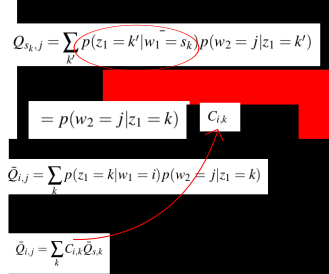
\includegraphics[scale=0.9]{pic2}
\end{figure}



\begin{frame}{Topic recovery using Bayes' Rule}


\framesubtitle{Convex Hull II}


\begin{figure}[H]
\begin{centering}
\includegraphics[scale=0.4]{convexhull}
\par\end{centering}

\protect\caption{Convex Hull}
\end{figure}

\begin{itemize}
\item Using this geometric simplification, we can determine the relevant
probabilities to allow us to use Bayes' Rule in the end.
\end{itemize}

\[
p(w_{1}=i|z_{1}=k)=\frac{p(z_{1}=k|w_{1}=i)p(w_{1}=i)}{\sum_{i}p(z_{1}=k|w_{1}=i')p(w_{1}=i')}\,\,\,\,\,(4)
\]


\end{frame}

\begin{frame}{Anchor words}


\framesubtitle{Finding anchor words}


\begin{figure}[H]
\begin{centering}
\includegraphics[scale=0.4]{convexhull}
\par\end{centering}

\protect\caption{Convex Hull}
\end{figure}

\begin{itemize}
\item Previous algorithm: tests whether each of the V points is a vertex
of the convex hull (and thus an anchor word) using the linear programming
technique

\begin{itemize}
\item Inefficient
\end{itemize}
\end{itemize}
\end{frame}

\begin{frame}{Anchor words}


\framesubtitle{Efficient algorithm}
\begin{itemize}
\item Iterative algorithm

\begin{itemize}
\item Finds farthest point from subspace spanned by anchor words so far
\item Farthest point will be the new anchor word
\end{itemize}
\item Finds anchor word most different from the ones found so far
\item Terminates when it has found K anchor (K is input to algorithm, \#
topics)\end{itemize}
\end{frame}

\end{document}
